% \documentclass[handout,xcolor=pdftex,dvipsnames,table]{beamer}

%\documentclass[aspectratio=169]{beamer} % WIDESCREEN
\documentclass[t]{beamer} % Aspecto 4:3

\usepackage[utf8]{inputenc}
\usepackage[T1]{fontenc}
\usepackage[english,brazil]{babel}
%\usepackage{natbib}

\usepackage{tikz}

% usando tema personalizado.
% arquivo beamerthemeUFFS.sty deve estar no mesmo diretório do .tex
\usepackage{beamerthemeUFFS}
\usepackage{ragged2e}
\usepackage{setspace}
\usepackage{animate}

\hypersetup{
    pdfstartview={Fit},
    pdftitle={Geração procedural de biomas},
 	pdfsubject={ApresentacaoDefesaTCC1},
 	pdfauthor={João Carlos Becker}
}

%%%%%%%%%%%%%%%%%%%%%%%%%%%%%%%%%%%%%%%%%%%%
 
\title{Geração procedural de biomas}
\author{João Carlos Becker} 

%\date{28 de junho de 2016}
\institute{Ciência da Computação\\
Universidade Federal da Fronteira Sul - Chapecó}

%%%%%%%%%%%%%%%%%%%%%%%%%%%%%%%%%%%%%%%%%%%%

\begin{document}

\setstretch{1} %espaçamento

\addtobeamertemplate{frametitle}{}{%
\begin{tikzpicture}[remember picture,overlay]
\node[anchor=north east,yshift=2pt] at (current page.north east) {
\includegraphics[height=1cm]{img/logo_curso}};
\end{tikzpicture}}

\setbeamertemplate{footline}{
	\color{white}
     \\
    }

\begin{frame}
	\maketitle
\end{frame}

\addtocounter{framenumber}{-1}

% Descomente as linhas abaixo se desejar colocar um sumário de todas as seções
%\begin{frame}[t]{Sumário}
%\tableofcontents
%\end{frame}
\setbeamertemplate{footline}{
    \color{black}
    \hfill \insertframenumber\,/\,\inserttotalframenumber~
}

%Utilizado para alinhar figuras
\setbeamertemplate{caption}{\raggedright\insertcaption\par}

\def\sectionname{}
\def\insertsectionnumber{}
\def\subsectionname{}
\def\insertsubsectionnumber{}

\AtBeginSection{\frame{\sectionpage}\addtocounter{framenumber}{-1}}


\AtBeginSubsection{\frame{\subsectionpage}\addtocounter{framenumber}{-1} }
\AtBeginSubsubsection{\frame{\subsubsectionpage}\addtocounter{framenumber}{-1} }


%%%%%%%%%%%%%%%%%%%%%%%%%%%%%%%%%%%%%%%%%%%%
% Inicio do documento
%%%%%%%%%%%%%%%%%%%%%%%%%%%%%%%%%%%%%%%%%%%%

\begin{frame}{Roteiro}
  \begin{itemize} \setlength\itemsep{1em}
    \item Objetivo.
    \item Perlin Noise
\end{itemize}
\end{frame}
%pdflatex apresentacao.tex 
%bibtex apresentacao.aux
%pdflatex apresentacao.tex 
%pdflatex apresentacao.tex 

\begin{frame}{Ruído de Perlin}
    \begin{itemize}\setlength\itemsep{1em}
        \item Falar sobre ruído de  \cite{perlin2002improving} aqui =D    
    \end{itemize}
    \begin{figure}[H]
        \centering
        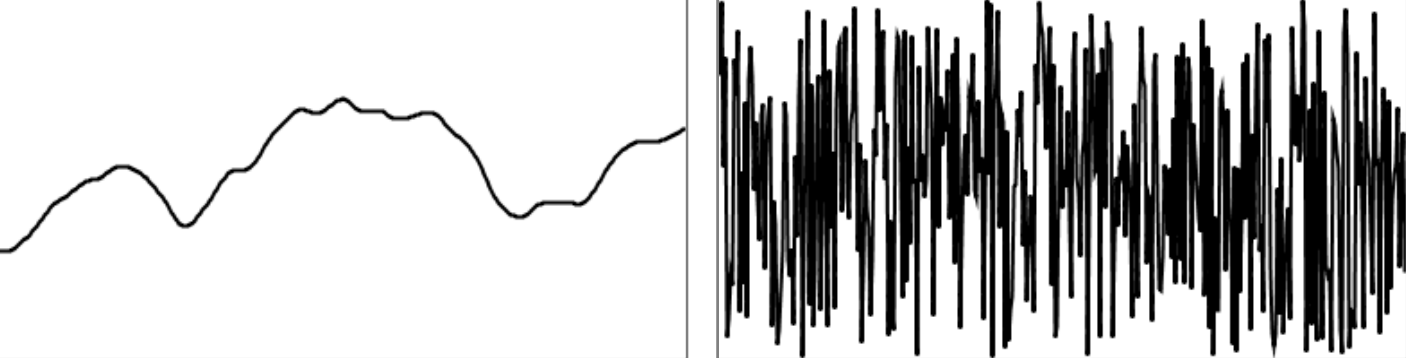
\includegraphics[width=.75\textwidth]{img/randomAndNoise}
        \caption{Da esquerda: Função de ruído e função que gera números aleatórios. Por \cite{shiffman2012nature}}
        \label{fig:randomAndNoise}
    \end{figure}
    
\end{frame}

\begin{frame}{Ruído de Perlin}
    \begin{itemize}\setlength\itemsep{1em}
        \item Falar sobre ruído de  
    \end{itemize}
    \begin{figure}[H]
        \centering
        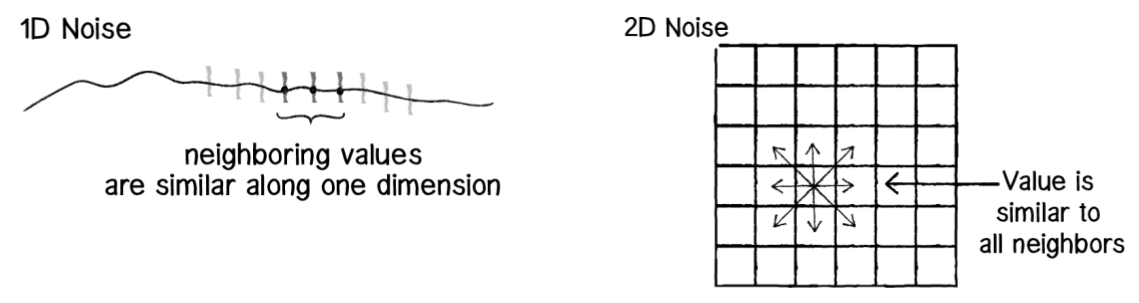
\includegraphics[width=.75\textwidth]{img/1dto2dnoise}
        \caption{À esquerda relação entre pontos unidimensionais, à direita bidimensionais. Por \cite{shiffman2012nature}}
        \label{fig:1dto2dnoise}
    \end{figure}
    
\end{frame}



\begin{frame}{Ruído de Perlin}
    
    \begin{figure}
        \centering
        \begin{subfigure}[b]{0.6\textwidth}
            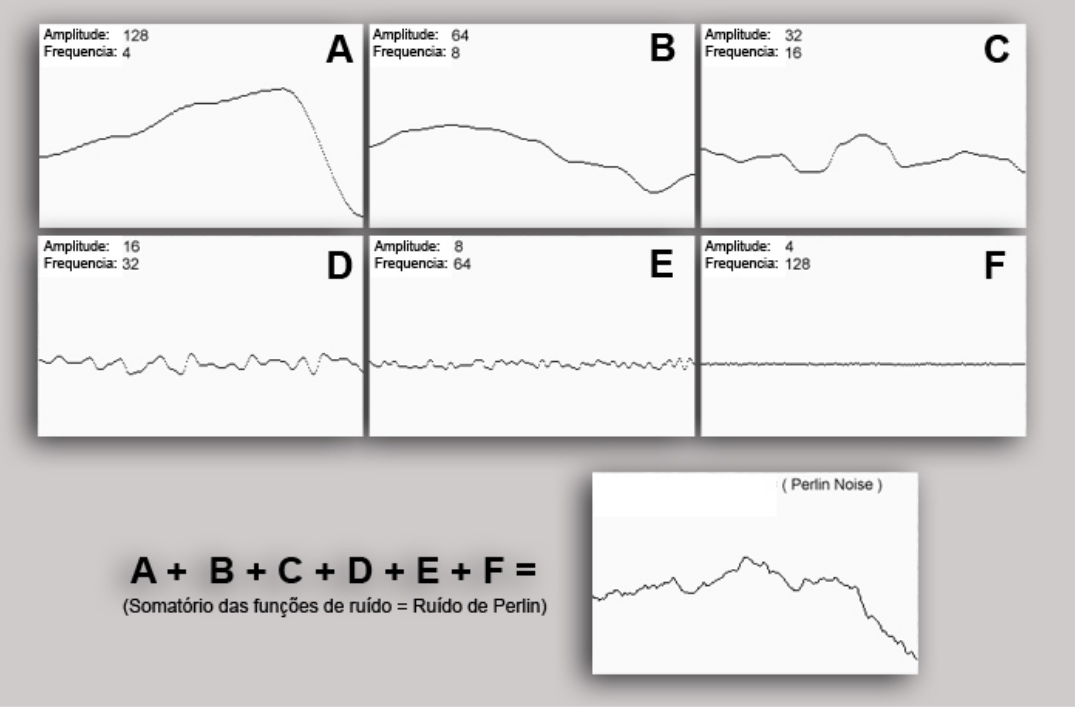
\includegraphics[width=\textwidth]{img/perlin1d}
            \caption{Ruído de Perlin com uma dimensão}
            \label{fig:perlin1d}
        \end{subfigure}
        ~ %add desired spacing between images, e. g. ~, \quad, \qquad, \hfill etc. 
          %(or a blank line to force the subfigure onto a new line)
        \begin{subfigure}[b]{0.35\textwidth}
            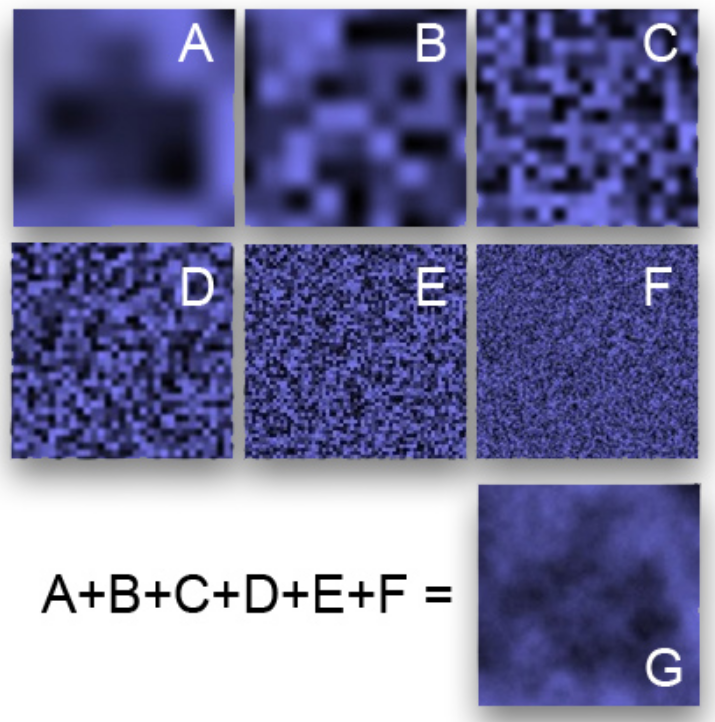
\includegraphics[width=\textwidth]{img/perlin2d}
            \caption{Ruído de Perlin com duas dimensões}
            \label{fig:perlin2d}
        \end{subfigure}
        ~ %add desired spacing between images, e. g. ~, \quad, \qquad, \hfill etc. 
        %(or a blank line to force the subfigure onto a new line)
        \caption{Perlin para uma e duas dimensões. Por \cite{elias2000perlin}}
        \label{fig:perlin1d2d}
    \end{figure}
    
\end{frame}



\setbeamertemplate{footline}{
	\color{white}
     \\
    }

\begin{frame}{Referências} % allowframebreaks -> Referências grandes
   \bibliography{referencias}
   \bibliographystyle{apalike}
\end{frame}

\begin{frame}
	\maketitle
\end{frame}

%% Coloquei o  livro em  anotacoes.bib. Pode incluir  outras referências
%% alí. (AG)

\end{document}
